%%%%%%%%%%%%%%%%%%%%%%%%%%%%%%%%%%%%%%%%%
% Beamer Presentation
% LaTeX Template
% Version 1.0 (10/11/12)
%
% This template has been downloaded from:
% http://www.LaTeXTemplates.com
%
% License:
% CC BY-NC-SA 3.0 (http://creativecommons.org/licenses/by-nc-sa/3.0/)
%
%%%%%%%%%%%%%%%%%%%%%%%%%%%%%%%%%%%%%%%%%

%----------------------------------------------------------------------------------------
%	PACKAGES AND THEMES
%----------------------------------------------------------------------------------------

\documentclass{beamer}

\mode<presentation> {

% The Beamer class comes with a number of default slide themes
% which change the colors and layouts of slides. Below this is a list
% of all the themes, uncomment each in turn to see what they look like.

%\usetheme{default}
%\usetheme{AnnArbor}
%\usetheme{Antibes}
%\usetheme{Bergen}
%\usetheme{Berkeley}
%\usetheme{Berlin}
%\usetheme{Boadilla}
%\usetheme{CambridgeUS}
%\usetheme{Copenhagen}
\usetheme{Darmstadt}
%\usetheme{Dresden}
%\usetheme{Frankfurt}
%\usetheme{Goettingen}
%\usetheme{Hannover}
%\usetheme{Ilmenau}
%\usetheme{JuanLesPins}
%\usetheme{Luebeck}
%\usetheme{Madrid}
%*\usetheme{Malmoe}
%\usetheme{Marburg}
%\usetheme{Montpellier}
%\usetheme{PaloAlto}
%\usetheme{Pittsburgh}
%\usetheme{Rochester}
%\usetheme{Singapore}
%\usetheme{Szeged}
%\usetheme{Warsaw}

% As well as themes, the Beamer class has a number of color themes
% for any slide theme. Uncomment each of these in turn to see how it
% changes the colors of your current slide theme.

%\usecolortheme{albatross}
%\usecolortheme{beaver}
%\usecolortheme{beetle}
%\usecolortheme{crane}
%\usecolortheme{dolphin}
%\usecolortheme{dove}
%\usecolortheme{fly}
%\usecolortheme{lily}
\usecolortheme{orchid}
%\usecolortheme{rose}
%\usecolortheme{seagull}
%\usecolortheme{seahorse}
%\usecolortheme{whale}
%\usecolortheme{wolverine}

%\setbeamertemplate{footline} % To remove the footer line in all slides uncomment this line
%\setbeamertemplate{footline}[page number] % To replace the footer line in all slides with a simple slide count uncomment this line

%\setbeamertemplate{navigation symbols}{} % To remove the navigation symbols from the bottom of all slides uncomment this line
}


\usepackage{graphicx} % Allows including images
\usepackage{booktabs} % Allows the use of \toprule, \midrule and \bottomrule in tables
\usepackage{xspace}
\usepackage{caption}
\usepackage{subfigure}
\usepackage[english,brazil]{babel}
\usepackage[utf8]{inputenc}

%Renomeia o nome padrao das figuras.
\renewcommand{\figurename}{Figura}
\renewcommand{\tablename}{Tabela}
%----------------------------------------------------------------------------------------
%	TITLE PAGE
%----------------------------------------------------------------------------------------

\title[Computação Gráfica]{Visualização - 3D} % The short title appears at the bottom of every slide, the full title is only on the title page

\author{Uéliton Freitas} % Your name
\institute[UFMS] % Your institution as it will appear on the bottom of every slide, may be shorthand to save space
{
Universidade Católica Dom Bosco - UCDB \\ % Your institution for the title page
\medskip
\textit{freitas.ueliton@gmail.com} % Your email address
}
\date{\today} % Date, can be changed to a custom date


\begin{document}

\begin{frame}
\titlepage % Print the title page as the first slide
\end{frame}

\begin{frame}
\frametitle{Sumário} % Table of contents slide, comment this block out to remove it
\tableofcontents % Throughout your presentation, if you choose to use \section{} and \subsection{} commands, these will automatically be printed on this slide as an overview of your presentation
\end{frame}




%----------------------------------------------------------------------------------------
%	PRESENTATION SLIDES
%----------------------------------------------------------------------------------------

%------------------------------------------------
\section{Introdução} 
%------------------------------------------------

%\section{Speeded-Up Robust Features - SURF} % A subsection can be created just before a set of slides with a common theme to further break down your presentation into chunks
%\section{Baf Of Features and Colors}

%\section{Refer\^encias}
%%%%%%%%%%%%%%%%%%%%%%%%%%%%%%%%%%%%%%%%%%%%%%%%%%%%%%%%%%%%%%%%%%%%%%%%%%%%%%%%%%%%%%%%%%
\begin{frame}
\frametitle{Introdução}


	\begin{block}{Visualização}
		\begin{itemize}
			\item<1-> As funções de visualização processam a descrição dos objetos por meio de vários procedimentos a fim de projetar a visão do objeto na superfície do dispositivo de saída.
			\item<2-> Alguns destes procedimentos são parecidos com com o Pipeline de visualização 2D
				\begin{itemize}
					\item Rotinas de recorte.
				\end{itemize}
			\item Mas há outras rotinas que são específicas do 3D.
			\begin{itemize}
				\item Rotinas de projeção.
				\item Identificação de partes visuais da cena.
				\item Efeitos de Luz.
			\end{itemize}							 		 
		\end{itemize}
	\end{block}
	
\end{frame}



%%%%%%%%%%%%%%%%%%%%%%%%%%%%%%%%%%%%%%%%%%%%%%%%%%%%%%%%%%%%%%%%%%%%%%%%%%%%%%%%%%%%%%%%%%
\begin{frame}
\frametitle{Introdução}


	\begin{block}{Visualização de uma Cena 3D}
		\begin{itemize}
			\item Primeiramente, para obter uma visão de uma cena 3D descritas nas \textbf{coordenadas do mundo}, é necessário definir um sistema de referência para os parâmetros de visão (Câmera).
		
			\begin{itemize}
				\item Definir a posição e orientação do \textbf{plano de visão} ou \textbf{plano de projeção}.
			\end{itemize}
		\end{itemize}
	\end{block}
	
	\begin{figure}[!h]
			\begin{center}
			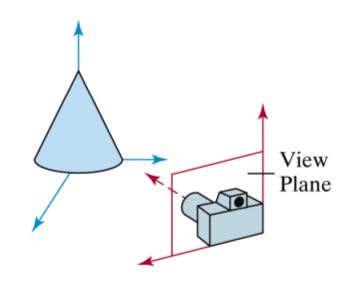
\includegraphics[width=0.5\textwidth]{Figures/ViePla}
			\end{center}
	\end{figure}	
\end{frame}


%%%%%%%%%%%%%%%%%%%%%%%%%%%%%%%%%%%%%%%%%%%%%%%%%%%%%%%%%%%%%%%%%%%%%%%%%%%%%%%%%%%%%%%%%%
\begin{frame}
\frametitle{Introdução}


	\begin{block}{Projeções}
		\begin{itemize}
			\item É possível escolher diferentes métodos para projetar uma cena de visão.
			\begin{itemize}
				\item \textbf{Projeção Paralela} - projeta objetos ao longo de linhas paralelas (Usado para desenhos arquitetônicos).
				\item \textbf{Projeção de Perspectiva} - projeta os pontos de um objeto ao longo de caminhos convergentes produzindo cenas mais realísticas (objetos longe do observador ficam menores).
			\end{itemize}
		\end{itemize}
	\end{block}
	
	\begin{figure}[!h]
			\begin{center}
			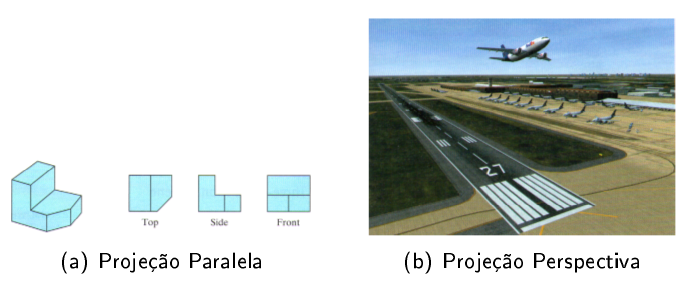
\includegraphics[width=0.5\textwidth]{Figures/Pro}
			\end{center}
	\end{figure}	
\end{frame}

%%%%%%%%%%%%%%%%%%%%%%%%%%%%%%%%%%%%%%%%%%%%%%%%%%%%%%%%%%%%%%%%%%%%%%%%%%%%%%%%%%%%%%%%%%
\begin{frame}
\frametitle{Introdução}


	\begin{block}{Profundidade}
		\begin{itemize}
			\item São raras as exceções em que a profundidade não é importante para composição de uma cena 3D.
			\item A profundidade explicita frente e trás do objeto.
		\end{itemize}
	\end{block}
	
	\begin{figure}[!h]
			\begin{center}
			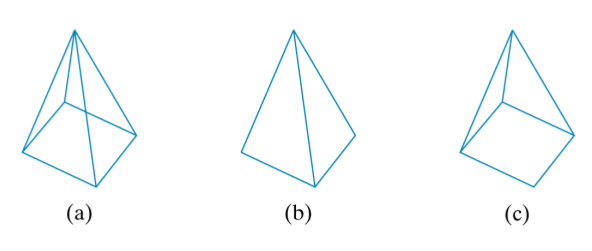
\includegraphics[width=0.5\textwidth]{Figures/ProObj}
			\caption{A Figura a possui problemas de visualização devido a falta de informação de profundidade}
			\end{center}
	\end{figure}	
\end{frame}


%%%%%%%%%%%%%%%%%%%%%%%%%%%%%%%%%%%%%%%%%%%%%%%%%%%%%%%%%%%%%%%%%%%%%%%%%%%%%%%%%%%%%%%%%%
\begin{frame}
\frametitle{Introdução}


	\begin{block}{Identificando Linhas e Superfícies Visíveis}
		\begin{itemize}
			\item Uma forma simples de resolver o problema de profundidade é de objetos aramados (wire-frames) é variar o brilho das linhas.
			\begin{itemize}
				\item Linhas mais próximas da posição de visão possuem maior brilho.
			\end{itemize}
		\end{itemize}
	\end{block}
	
	\begin{figure}[!h]
			\begin{center}
			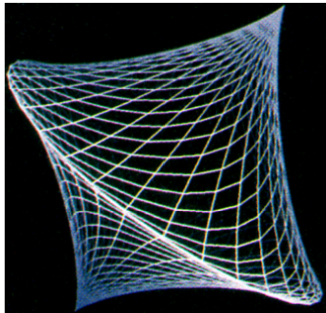
\includegraphics[width=0.3\textwidth]{Figures/WirFra}
			\end{center}
	\end{figure}	
\end{frame}





%%%%%%%%%%%%%%%%%%%%%%%%%%%%%%%%%%%%%%%%%%%%%%%%%%%%%%%%%%%%%%%%%%%%%%%%%%%%%%%%%%%%%%%%%%
\begin{frame}
\frametitle{Introdução}


	\begin{block}{Cenas Wire-Frame}
		\begin{itemize}
			\item Há vários métodos para definir a profundidade de um objeto wire-frame.
			\begin{itemize}
				\item Cores diferentes para linhas visíveis e não visíveis.
				\item Mostrar linhas não visíveis como linhas pontilhadas.
			\end{itemize}
		\end{itemize}
	\end{block}
	
	\begin{block}{Cenas Realísticas}
		\begin{itemize}
			\item As partes dos objetos que não são vistas são completamente eliminadas.
			\begin{itemize}
				\item Os pixels da tela terão informações apenas das cores da superfície da frente.
			\end{itemize}
		\end{itemize}
	\end{block}
\end{frame}




%%%%%%%%%%%%%%%%%%%%%%%%%%%%%%%%%%%%%%%%%%%%%%%%%%%%%%%%%%%%%%%%%%%%%%%%%%%%%%%%%%%%%%%%%%
\begin{frame}
\frametitle{Introdução}


	\begin{block}{Rendering de Superfície}
		\begin{itemize}
			\item Efeitos realísticos das cenas são objetos usando efeitos de iluminação
			\begin{itemize}
				\item Define-se a luz do ambiente.
				\item Define-se a cor e posição das fontes de luz.
			\end{itemize}
			\item Também são definidos o material que os objetos são constituídos.
			\begin{itemize}
				\item Transparentes, rugosos, opacos, reflexivos, etc.
			\end{itemize}
		\end{itemize}
	\end{block}
	
	\begin{figure}[!h]
			\begin{center}
			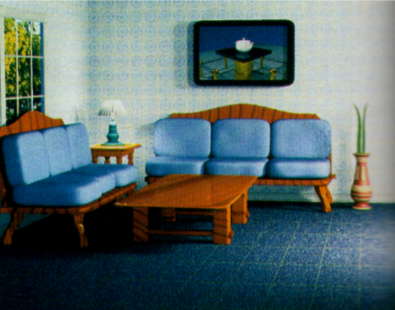
\includegraphics[width=0.38\textwidth]{Figures/Cen}
			\end{center}
	\end{figure}	
\end{frame}

%%%%%%%%%%%%%%%%%%%%%%%%%%%%%%%%%%%%%%%%%%%%%%%%%%%%%%%%%%%%%%%%%%%%%%%%%%%%%%%%%%%%%%%%%%
\section{Viewing Pipeline 3D}
\begin{frame}
\frametitle{Introdução}


	\begin{block}{Criando uma Imagem}
		\begin{itemize}
			\item O processo para criar uma imagem em computação gráfica em uma cena 3D é semelhante a tirar uma foto.
			\begin{itemize}
				\item Define-se a posição de visão da câmera.
				\item Define-se a orientação da câmera.
				\begin{itemize}
					\item Como a câmera estará apontada a partir da posição de visão.
					\item COmo a câmera vai rotacionar definindo a posição \textbf{up}.
				\end{itemize}
			\end{itemize}
		\end{itemize}
	\end{block}
	
	\begin{figure}[!h]
			\begin{center}
			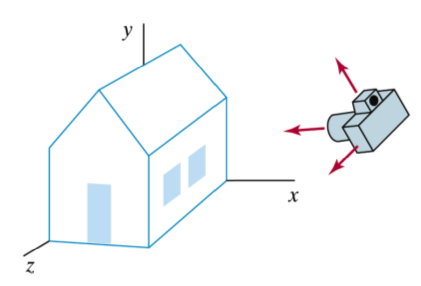
\includegraphics[width=0.5\textwidth]{Figures/CamPos}
			\end{center}
	\end{figure}	
\end{frame}

%%%%%%%%%%%%%%%%%%%%%%%%%%%%%%%%%%%%%%%%%%%%%%%%%%%%%%%%%%%%%%%%%%%%%%%%%%%%%%%%%%%%%%%%%%
\begin{frame}
\frametitle{Introdução}


	\begin{block}{Criando uma Imagem}
		\begin{itemize}
			\item<1-> Há algumas semelhanças entre o \textit{Pipeline da Viewing 2D e 3D}.
			\begin{itemize}
				\item Uma \textbf{viewport 2D} é utilizada para posicionar a visão projetada no dispositivo de saída.
				\item  Uma janela de recorte 2D é utilizada para selecionar o que será visto na cena e mapeado para viewport.
			\end{itemize}
			\item<2-> Porém há algumas diferenças
			\begin{itemize}
				\item A janela de recorte é posicionada sobre um plano de visão.
				\item A cena é recortada considerando um volume no espaço (volume de recorte) usando planos de recorte.
			\end{itemize}
		\end{itemize}
	\end{block}
\end{frame}

%----------------------------------------------------------------------------------------

\end{document} 